\begin{wrapfigure}[0]{r}[0cm]{4cm}
 \vspace{-6cm}
  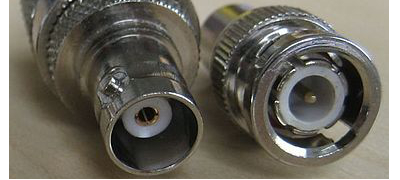
\includegraphics[scale=0.4]{KabelLeitungen/Bilder/bnc.jpg}
 \vspace{-6cm}
\end{wrapfigure}

\section*{Theorie- und Prüfungsfragen}

%--------------------------------------------


\mucho{1}{TH303}
{Im Amateurfunk übliche Koaxialkabel weisen typischerweise Wellenwiderstände von}%Frage
{50, 60 und 75 $\Omega$ auf.}%A
{50, 300 und 600 $\Omega$ auf.}%B
{60, 120 und 240 $\Omega$ auf.}%C
{50, 75 und 240 $\Omega$ auf.}%D
{A}%Lösung

\mucho{2}{TH316}
{Eine offene Paralleldrahtleitung ist aus Draht mit einem Durchmesser von 2 mm gefertigt. Der Abstand der Leiter beträgt 20 cm. Wie hoch ist der Wellenwiderstand der Leitung?}%Frage
{ca. 276 $\Omega$}%A
{ca. 635 $\Omega$}%B
{ca. 820 $\Omega$}%C
{ca. 2,8k $\Omega$}%D
{B; $Z_W = \dfrac{120\Omega}{1} \cdot ln \left( \dfrac{2\cdot 200mm}{2mm} \right) = 635,7\Omega$; für Luft $e_r=1$}%Lösung

\mucho{3}{TH313}
{Wann ist eine Speiseleitung asymmetrisch?}%Frage
{Wenn die beiden Leiter unterschiedlich geformt sind, z.B. Koaxialkabel.}%A
{Wenn die hin- und zurücklaufende Leistung verschieden sind.}%B
{Wenn sie außerhalb ihrer Resonanzfrequenz betrieben wird.}%C
{Wenn die Koaxial-Leitung Spannung gegen Erde führt.}%D
{A}%Lösung

\mucho{4}{TH314}
{Bei einer Leitung mit symmetrischer Übertragung}%Frage
{sind die Impedanzen bei beiden Leitern gegen Erde unendlich hoch.}%A
{liegt einer der beiden Leiter auf Erdpotential.}%B
{ist Strom und Spannung in den beiden Leitern gegenüber Erde gleich groß und gegenphasig.}%C
{ist Strom und Spannung in den beiden Leitern gegenüber Erde gleich groß und gleichphasig.}%D
{C}%Lösung

\mucho{5}{TH324}
{Welche Leitungen sollten für die HF-Verbindungen zwischen Einrichtungen in der Amateurfunkstelle verwendet werden, um unerwünschte Abstrahlungen zu vermeiden?}%Frage
{Unabgestimmte Speiseleitungen}%A
{Symmetrische Feederleitungen}%B
{Hochwertige asymmetrische Koaxialkabel}%C
{Hochwertige abgeschirmte Netzanschlusskabel}%D
{C}%Lösung

\mucho{6}{TH320}
{Der Verkürzungsfaktor eines Koaxialkabels mit einem Dielektrikum aus massivem Polyäthylen beträgt ungefähr}%Frage
{0,66.}%A
{0,1.}%B
{0,8.}%C
{1,0.}%D
{A; $k=\dfrac{1}{\sqrt{\epsilon_r}} = \dfrac{1}{\sqrt{2,29}} = \dfrac{1}{1,513} = 0,66  $}%Lösung

\mucho{7}{TH319}
{Der Verkürzungsfaktor einer luftisolierten Paralleldrahtleitung ist}%Frage
{0,1.}%A
{ungefähr 1}%B
{0,66.}%C
{unbestimmt}%D
{B}%Lösung

\mucho{8}{TH322}
{Welche mechanische Länge hat ein $\lambda/4$ langes Koaxkabel mit Vollpolyethylenisolierung bei 145 MHz?}%Frage
{17 cm}%A
{34,2 cm}%B
{51,7 cm}%C
{1,03 m}%D
{B; $ 
\lambda = \dfrac{300m}{f} = \dfrac{300}{145} = 2,069m; 
l_{Luft} = \dfrac{ \lambda }{4}=0,517m; 
l= 0,66 \cdot 0,517m = 34,12 cm $}%Lösung

\mucho{9}{TH306}
{Welche Dämpfung ergibt sich auf der Grundlage des Kabeldämpfungsdiagramms für ein 25-m-langes Koaxialkabel vom Typ RG213 (MIL) bei 3,5 MHz?}%Frage
{0,1 dB}%A
{1,2 dB}%B
{0,6 dB}%C
{0,3 dB}%D
{D}%Lösung

\mucho{10}{TH307}
{Welche Dämpfung ergibt sich auf der Grundlage des Kabeldämpfungsdiagramms für ein 25-m-langes Koaxialkabel vom Typ RG213U-S100 bei 29 MHz?}%Frage
{0,5 dB}%A
{2,1 dB}%B
{1,1 dB}%C
{0,2 dB}%D
{A}%Lösung

\mucho{11}{TH311}
{Welches der folgenden Kabel weist im Kurzwellenbereich den geringsten Verlust auf?}%Frage
{Kunststoffisolierte Zweidrahtleitung}%A
{Koaxialkabel mit Vollisolation}%B
{UKW-Bandleitung}%C
{Offene Zweidrahtleitung}%D
{D}%Lösung